\section{Development/Implementation View}

The development view describes the software architecture and implementation details of the Smart Parking IoT system. The system follows a layered architecture pattern with clear separation of concerns.

\subsection{Architecture Overview}

\begin{figure}[H]
\centering
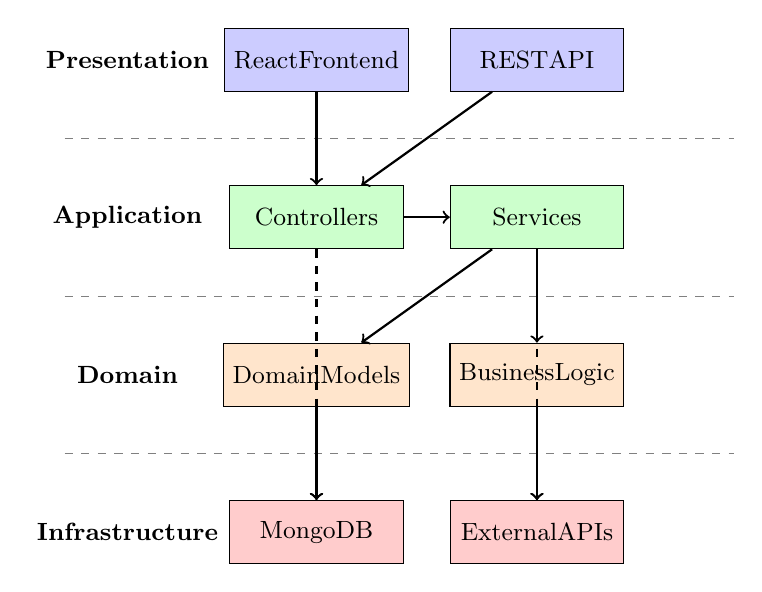
\begin{tikzpicture}[auto, font=\small]
    % Layer labels on the left
    \node at (-3.2,5.5) {\textbf{Presentation}};
    \node at (-3.2,3.5) {\textbf{Application}};
    \node at (-3.2,1.5) {\textbf{Domain}};
    \node at (-3.2,-0.5) {\textbf{Infrastructure}};

    % Presentation Layer Components
    \node[draw, fill=blue!20, minimum width=2.2cm, minimum height=0.8cm, text centered] (frontend) at (-0.8,5.5) {React\newline Frontend};
    \node[draw, fill=blue!20, minimum width=2.2cm, minimum height=0.8cm, text centered] (api) at (2,5.5) {REST\newline API};

    % Application Layer Components
    \node[draw, fill=green!20, minimum width=2.2cm, minimum height=0.8cm] (controllers) at (-0.8,3.5) {Controllers};
    \node[draw, fill=green!20, minimum width=2.2cm, minimum height=0.8cm] (services) at (2,3.5) {Services};

    % Domain Layer Components
    \node[draw, fill=orange!20, minimum width=2.2cm, minimum height=0.8cm, text centered] (models) at (-0.8,1.5) {Domain\newline Models};
    \node[draw, fill=orange!20, minimum width=2.2cm, minimum height=0.8cm, text centered] (business) at (2,1.5) {Business\newline Logic};

    % Infrastructure Layer Components
    \node[draw, fill=red!20, minimum width=2.2cm, minimum height=0.8cm] (database) at (-0.8,-0.5) {MongoDB};
    \node[draw, fill=red!20, minimum width=2.2cm, minimum height=0.8cm, text centered] (external) at (2,-0.5) {External\newline APIs};

    % Layer separators (light lines)
    \draw[gray, dashed, very thin] (-4,4.5) -- (4.5,4.5);
    \draw[gray, dashed, very thin] (-4,2.5) -- (4.5,2.5);
    \draw[gray, dashed, very thin] (-4,0.5) -- (4.5,0.5);

    % Connections within and between layers
    \draw[->, thick] (frontend) -- (controllers);
    \draw[->, thick] (api) -- (controllers);
    \draw[->, thick] (controllers) -- (services);
    \draw[->, thick] (services) -- (models);
    \draw[->, thick] (services) -- (business);
    \draw[->, thick] (models) -- (database);
    \draw[->, thick] (business) -- (external);

    % Cross-layer connections
    \draw[->, thick, dashed] (controllers) -- (database);
    \draw[->, thick, dashed] (services) -- (external);
\end{tikzpicture}
\caption{Layered Architecture Overview}
\label{fig:layered-arch}
\end{figure}

\subsection{Technology Stack}

\subsubsection{Backend Technology Stack}
\begin{table}[H]
\centering
\small
\renewcommand{\arraystretch}{1.3}
\begin{tabularx}{\textwidth}{|l|l|>{\RaggedRight\arraybackslash}X|}
\hline
\textbf{Layer} & \textbf{Technology} & \textbf{Purpose} \\
\hline
Runtime & Node.js 18+ & JavaScript runtime environment \\
\hline
Framework & Express 5 & Web application framework \\
\hline
Language & TypeScript & Type-safe JavaScript development \\
\hline
Database & MongoDB & NoSQL document database \\
\hline
ODM & Mongoose & MongoDB object modeling \\
\hline
Authentication & JWT & Token-based authentication \\
\hline
Logging & Pino & High-performance logging \\
\hline
API Documentation & Swagger/OpenAPI & API specification and testing \\
\hline
Testing & Jest & Unit and integration testing \\
\hline
Linting & ESLint & Code quality and style checking \\
\hline
\end{tabularx}
\caption{Backend Technology Stack}
\label{tab:backend-stack}
\end{table}

\subsubsection{Frontend Technology Stack}
\begin{table}[H]
\centering
\small
\renewcommand{\arraystretch}{1.3}
\begin{tabularx}{\textwidth}{|l|l|>{\RaggedRight\arraybackslash}X|}
\hline
\textbf{Layer} & \textbf{Technology} & \textbf{Purpose} \\
\hline
Framework & React 18 & Component-based UI library \\
\hline
Build Tool & Vite & Fast build tool and dev server \\
\hline
Language & TypeScript & Type-safe JavaScript development \\
\hline
Styling & Tailwind CSS v4 & Utility-first CSS framework \\
\hline
UI Components & Radix UI & Accessible component primitives \\
\hline
Routing & React Router & Client-side routing \\
\hline
Charts & Recharts & Data visualization components \\
\hline
State Management & React Context & Global state management \\
\hline
Testing & Vitest & Fast unit testing framework \\
\hline
Linting & ESLint & Code quality checking \\
\hline
\end{tabularx}
\caption{Frontend Technology Stack}
\label{tab:frontend-stack}
\end{table}

\subsection{Package Structure}

\subsubsection{Backend Package Structure}
\begin{figure}[H]
\centering
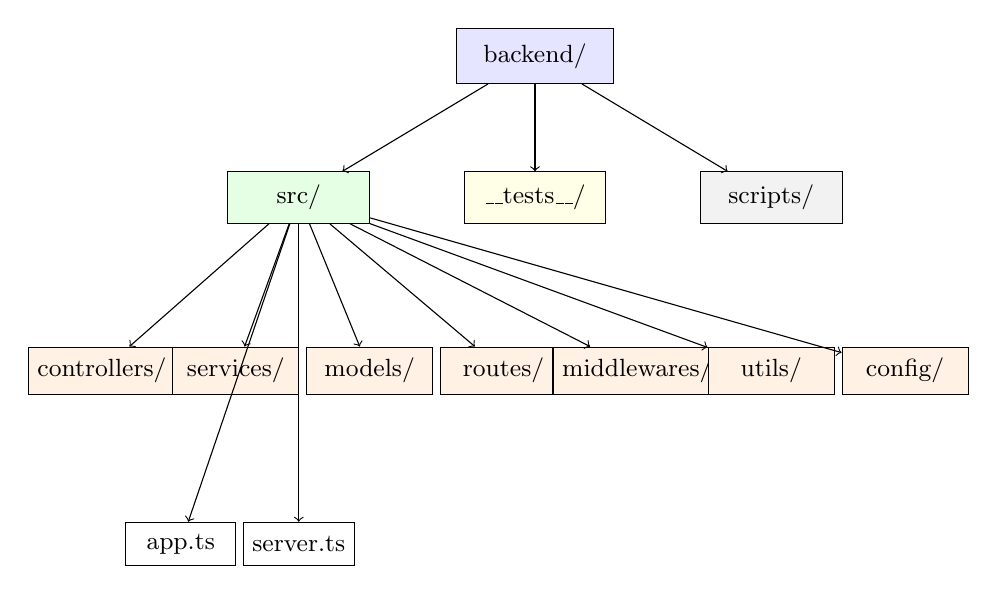
\begin{tikzpicture}[node distance=0.8cm, auto, font=\small]
    % Root
    \node[draw, fill=blue!10, minimum width=2cm, minimum height=0.7cm] (backend) at (0,7) {backend/};

    % Main directories - tier 1
    \node[draw, fill=green!10, minimum width=1.8cm, minimum height=0.65cm] (src) at (-3,5.2) {src/};
    \node[draw, fill=yellow!10, minimum width=1.8cm, minimum height=0.65cm] (tests) at (0,5.2) {\_\_tests\_\_/};
    \node[draw, fill=gray!10, minimum width=1.8cm, minimum height=0.65cm] (scripts) at (3,5.2) {scripts/};

    % src subdirectories - tier 2
    \node[draw, fill=orange!10, minimum width=1.6cm, minimum height=0.6cm] (controllers) at (-5.5,3) {controllers/};
    \node[draw, fill=orange!10, minimum width=1.6cm, minimum height=0.6cm] (services) at (-3.8,3) {services/};
    \node[draw, fill=orange!10, minimum width=1.6cm, minimum height=0.6cm] (models) at (-2.1,3) {models/};
    \node[draw, fill=orange!10, minimum width=1.6cm, minimum height=0.6cm] (routes) at (-0.4,3) {routes/};
    \node[draw, fill=orange!10, minimum width=1.6cm, minimum height=0.6cm] (middlewares) at (1.3,3) {middlewares/};
    \node[draw, fill=orange!10, minimum width=1.6cm, minimum height=0.6cm] (utils) at (3,3) {utils/};
    \node[draw, fill=orange!10, minimum width=1.6cm, minimum height=0.6cm] (config) at (4.7,3) {config/};

    % Files - tier 3
    \node[draw, fill=white, minimum width=1.4cm, minimum height=0.55cm] (app) at (-4.5,0.8) {app.ts};
    \node[draw, fill=white, minimum width=1.4cm, minimum height=0.55cm] (server) at (-3,0.8) {server.ts};

    % Connections from root
    \draw[->] (backend) -- (src);
    \draw[->] (backend) -- (tests);
    \draw[->] (backend) -- (scripts);

    % Connections from src
    \draw[->] (src) -- (controllers);
    \draw[->] (src) -- (services);
    \draw[->] (src) -- (models);
    \draw[->] (src) -- (routes);
    \draw[->] (src) -- (middlewares);
    \draw[->] (src) -- (utils);
    \draw[->] (src) -- (config);

    % Connections to files
    \draw[->] (src) -- (app);
    \draw[->] (src) -- (server);
\end{tikzpicture}
\caption{Backend Package Structure}
\label{fig:backend-structure}
\end{figure}

\subsubsection{Frontend Package Structure}
\begin{figure}[H]
\centering
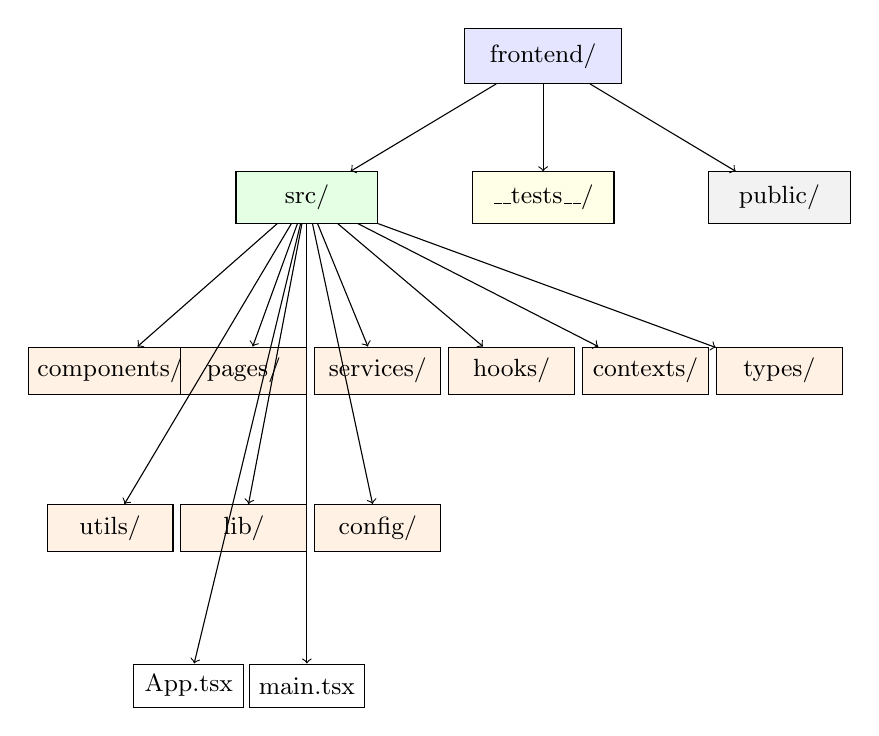
\begin{tikzpicture}[node distance=0.8cm, auto, font=\small]
    % Root
    \node[draw, fill=blue!10, minimum width=2cm, minimum height=0.7cm] (frontend) at (0,7) {frontend/};

    % Main directories - tier 1
    \node[draw, fill=green!10, minimum width=1.8cm, minimum height=0.65cm] (src) at (-3,5.2) {src/};
    \node[draw, fill=yellow!10, minimum width=1.8cm, minimum height=0.65cm] (tests) at (0,5.2) {\_\_tests\_\_/};
    \node[draw, fill=gray!10, minimum width=1.8cm, minimum height=0.65cm] (public) at (3,5.2) {public/};

    % src subdirectories - tier 2 (top row)
    \node[draw, fill=orange!10, minimum width=1.6cm, minimum height=0.6cm] (components) at (-5.5,3) {components/};
    \node[draw, fill=orange!10, minimum width=1.6cm, minimum height=0.6cm] (pages) at (-3.8,3) {pages/};
    \node[draw, fill=orange!10, minimum width=1.6cm, minimum height=0.6cm] (services) at (-2.1,3) {services/};
    \node[draw, fill=orange!10, minimum width=1.6cm, minimum height=0.6cm] (hooks) at (-0.4,3) {hooks/};
    \node[draw, fill=orange!10, minimum width=1.6cm, minimum height=0.6cm] (contexts) at (1.3,3) {contexts/};
    \node[draw, fill=orange!10, minimum width=1.6cm, minimum height=0.6cm] (types) at (3,3) {types/};

    % src subdirectories - tier 2 (bottom row)
    \node[draw, fill=orange!10, minimum width=1.6cm, minimum height=0.6cm] (utils) at (-5.5,1) {utils/};
    \node[draw, fill=orange!10, minimum width=1.6cm, minimum height=0.6cm] (lib) at (-3.8,1) {lib/};
    \node[draw, fill=orange!10, minimum width=1.6cm, minimum height=0.6cm] (config) at (-2.1,1) {config/};

    % Files - tier 3
    \node[draw, fill=white, minimum width=1.4cm, minimum height=0.55cm] (app) at (-4.5,-1) {App.tsx};
    \node[draw, fill=white, minimum width=1.4cm, minimum height=0.55cm] (main) at (-3,-1) {main.tsx};

    % Connections from root
    \draw[->] (frontend) -- (src);
    \draw[->] (frontend) -- (tests);
    \draw[->] (frontend) -- (public);

    % Connections from src to tier 2 (top row)
    \draw[->] (src) -- (components);
    \draw[->] (src) -- (pages);
    \draw[->] (src) -- (services);
    \draw[->] (src) -- (hooks);
    \draw[->] (src) -- (contexts);
    \draw[->] (src) -- (types);

    % Connections from src to tier 2 (bottom row)
    \draw[->] (src) -- (utils);
    \draw[->] (src) -- (lib);
    \draw[->] (src) -- (config);

    % Connections to files
    \draw[->] (src) -- (app);
    \draw[->] (src) -- (main);
\end{tikzpicture}
\caption{Frontend Package Structure}
\label{fig:frontend-structure}
\end{figure}

\subsection{Data Flow Architecture}

\subsubsection{Authentication Flow}
\begin{enumerate}
\item User submits credentials via frontend form
\item Frontend calls authentication API endpoint
\item Backend validates credentials against HCMUT SSO
\item JWT token generated and returned to frontend
\item Frontend stores token in local storage/context
\item Subsequent API calls include JWT in Authorization header
\end{enumerate}

\subsubsection{Parking Session Flow}
\begin{enumerate}
\item IoT sensor detects vehicle entry (planned) or manual check-in
\item Frontend sends check-in request to backend
\item Backend validates user permissions and zone capacity
\item ParkingSession document created in MongoDB
\item Zone capacity updated (denormalized for performance)
\item Real-time updates sent to connected clients via SSE
\end{enumerate}

\subsubsection{Billing and Payment Flow}
\begin{enumerate}
\item User initiates payment or system triggers billing cycle
\item Backend calculates fees based on pricing policies
\item Invoice created and stored in MongoDB
\item Payment request sent to BKPay gateway
\item Payment status updated in database
\item Confirmation sent to user via frontend
\end{enumerate}

\subsection{Component Relationships}

\subsubsection{Backend Component Dependencies}
\begin{itemize}
\item \textbf{Controllers} depend on Services and Models
\item \textbf{Services} contain business logic and orchestrate Models
\item \textbf{Models} define data schemas and database operations
\item \textbf{Middlewares} handle cross-cutting concerns (auth, logging, CORS)
\item \textbf{Routes} map URLs to controller methods
\end{itemize}

\subsubsection{Frontend Component Dependencies}
\begin{itemize}
\item \textbf{Pages} use Components and Hooks
\item \textbf{Components} consume Contexts and Services
\item \textbf{Hooks} manage state and side effects
\item \textbf{Contexts} provide global state management
\item \textbf{Services} handle API communication
\end{itemize}

\subsection{Design Patterns}

\subsubsection{Backend Patterns}
\begin{itemize}
\item \textbf{Layered Architecture:} Clear separation between presentation, application, domain, and infrastructure layers
\item \textbf{Dependency Injection:} Services injected into controllers
\item \textbf{Repository Pattern:} Models encapsulate data access logic
\item \textbf{Middleware Pattern:} Cross-cutting concerns handled by Express middleware
\item \textbf{Observer Pattern:} Event-driven architecture for real-time updates
\end{itemize}

\subsubsection{Frontend Patterns}
\begin{itemize}
\item \textbf{Component Composition:} Reusable UI components built from primitives
\item \textbf{Hooks Pattern:} Custom hooks for stateful logic reuse
\item \textbf{Context Pattern:} Global state management for authentication and app state
\item \textbf{Routing Pattern:} Declarative routing with React Router
\item \textbf{Container/Presentational:} Separation of data fetching and presentation logic
\end{itemize}

\subsection{Development Workflow}

\subsubsection{Backend Development}
\begin{enumerate}
\item Define Mongoose schemas in Models
\item Implement business logic in Services
\item Create API endpoints in Controllers
\item Configure routes and middleware
\item Write unit tests with Jest
\item Run linting and formatting checks
\end{enumerate}

\subsubsection{Frontend Development}
\begin{enumerate}
\item Define TypeScript interfaces in types/
\item Create reusable components in components/
\item Implement page layouts in pages/
\item Add state management with hooks and contexts
\item Integrate API calls via services/
\item Write unit tests with Vitest
\end{enumerate}